
 Putting together the components we have just explored and using the following values for the parameters, we can run the model using the code in Listing \ref{lst:part1}. This codes sets up the configuration for the scene and uses \texttt{ode45} to solve the ODE. The \texttt{MaxStep} option is used on the ODE solver to ensure that time increments of no more than \texttt{0.1} are used since the fox is continuously changing direction depending on its target and its essential to ensure these checks are done often to guarantee the accuracy of the model. Of course, it is also vital we do not make this value too small as this would negatively impact performance (in terms of speed). The value \texttt{0.1} was chosen as it produces a seemingly accurate simulation while not taking too long to complete the computation.
 
 The results are displayed in Figures \ref{output:simple} and  \ref{fig:simplegraph}. As we can see, the fox fails to catch the rabbit in these conditions. The \texttt{plotScene} function is included in Appendix \ref{ap:plotScene} in Listing \ref{lst:plotScene} for completeness.
 
 \begin{table}[h]
 \centering
\begin{tabular}{ll}
\textbf{Parameter} & \textbf{Value}       \\
$NW$      & (200, 0)    \\
$SW$      & (200, -400) \\
$R$       & (0, 0)      \\
$F$       & (250, -550) \\
$B$       & (600, 600)  \\
$s_{r0}$  & 13m/s       \\
$s_{f0}$  & 16m/s      
\end{tabular}
\end{table}

 \lstinputlisting[label={lst:part1}, caption={The code to run the model with a set of parameters.}] {../part1.m}
 
 \begin{figure}[h]
 \caption{The output from running the simple model.}
 \label{output:simple}
 \begin{verbatim}
>> part1

At time 65.263703, the rabbit reached the burrow.

 \end{verbatim}
 \end{figure}

\begin{figure}[h]
\centering

   \caption{The paths of the fox and rabbit under this configuration.}
   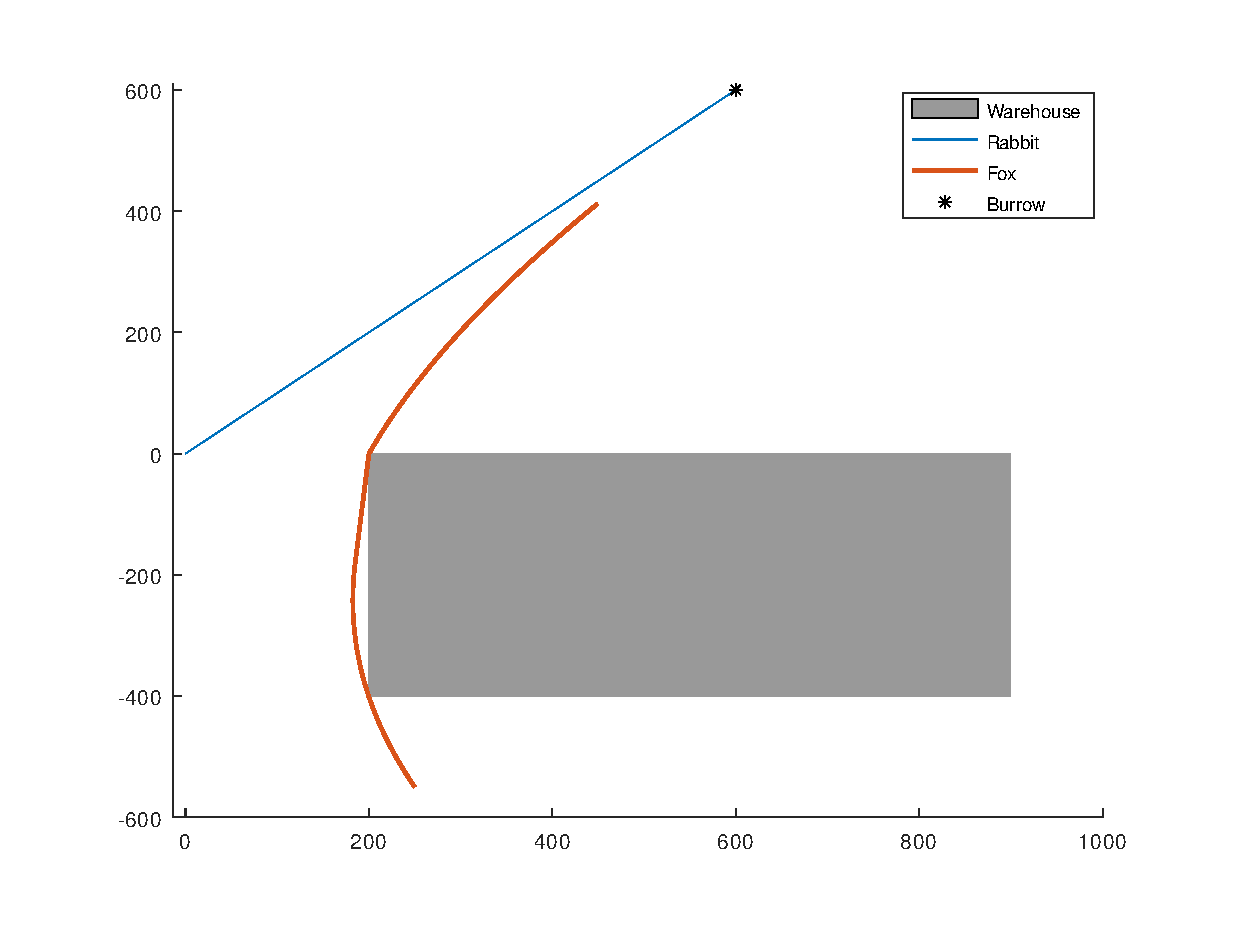
\includegraphics[scale=0.5]{simpleModel.eps}

      \label{fig:simplegraph}
\end{figure}
